% Options for packages loaded elsewhere
\PassOptionsToPackage{unicode}{hyperref}
\PassOptionsToPackage{hyphens}{url}
%
\documentclass[
]{article}
\usepackage{amsmath,amssymb}
\usepackage{lmodern}
\usepackage{iftex}
\ifPDFTeX
  \usepackage[T1]{fontenc}
  \usepackage[utf8]{inputenc}
  \usepackage{textcomp} % provide euro and other symbols
\else % if luatex or xetex
  \usepackage{unicode-math}
  \defaultfontfeatures{Scale=MatchLowercase}
  \defaultfontfeatures[\rmfamily]{Ligatures=TeX,Scale=1}
\fi
% Use upquote if available, for straight quotes in verbatim environments
\IfFileExists{upquote.sty}{\usepackage{upquote}}{}
\IfFileExists{microtype.sty}{% use microtype if available
  \usepackage[]{microtype}
  \UseMicrotypeSet[protrusion]{basicmath} % disable protrusion for tt fonts
}{}
\makeatletter
\@ifundefined{KOMAClassName}{% if non-KOMA class
  \IfFileExists{parskip.sty}{%
    \usepackage{parskip}
  }{% else
    \setlength{\parindent}{0pt}
    \setlength{\parskip}{6pt plus 2pt minus 1pt}}
}{% if KOMA class
  \KOMAoptions{parskip=half}}
\makeatother
\usepackage{xcolor}
\IfFileExists{xurl.sty}{\usepackage{xurl}}{} % add URL line breaks if available
\IfFileExists{bookmark.sty}{\usepackage{bookmark}}{\usepackage{hyperref}}
\hypersetup{
  pdftitle={Pràctica 2: Neteja i anàlisi de les dades},
  pdfauthor={Adrián Alonso Gonzalo i Alexandre Vidal De Palol},
  hidelinks,
  pdfcreator={LaTeX via pandoc}}
\urlstyle{same} % disable monospaced font for URLs
\usepackage[margin=1in]{geometry}
\usepackage{color}
\usepackage{fancyvrb}
\newcommand{\VerbBar}{|}
\newcommand{\VERB}{\Verb[commandchars=\\\{\}]}
\DefineVerbatimEnvironment{Highlighting}{Verbatim}{commandchars=\\\{\}}
% Add ',fontsize=\small' for more characters per line
\usepackage{framed}
\definecolor{shadecolor}{RGB}{48,48,48}
\newenvironment{Shaded}{\begin{snugshade}}{\end{snugshade}}
\newcommand{\AlertTok}[1]{\textcolor[rgb]{1.00,0.81,0.69}{#1}}
\newcommand{\AnnotationTok}[1]{\textcolor[rgb]{0.50,0.62,0.50}{\textbf{#1}}}
\newcommand{\AttributeTok}[1]{\textcolor[rgb]{0.80,0.80,0.80}{#1}}
\newcommand{\BaseNTok}[1]{\textcolor[rgb]{0.86,0.64,0.64}{#1}}
\newcommand{\BuiltInTok}[1]{\textcolor[rgb]{0.80,0.80,0.80}{#1}}
\newcommand{\CharTok}[1]{\textcolor[rgb]{0.86,0.64,0.64}{#1}}
\newcommand{\CommentTok}[1]{\textcolor[rgb]{0.50,0.62,0.50}{#1}}
\newcommand{\CommentVarTok}[1]{\textcolor[rgb]{0.50,0.62,0.50}{\textbf{#1}}}
\newcommand{\ConstantTok}[1]{\textcolor[rgb]{0.86,0.64,0.64}{\textbf{#1}}}
\newcommand{\ControlFlowTok}[1]{\textcolor[rgb]{0.94,0.87,0.69}{#1}}
\newcommand{\DataTypeTok}[1]{\textcolor[rgb]{0.87,0.87,0.75}{#1}}
\newcommand{\DecValTok}[1]{\textcolor[rgb]{0.86,0.86,0.80}{#1}}
\newcommand{\DocumentationTok}[1]{\textcolor[rgb]{0.50,0.62,0.50}{#1}}
\newcommand{\ErrorTok}[1]{\textcolor[rgb]{0.76,0.75,0.62}{#1}}
\newcommand{\ExtensionTok}[1]{\textcolor[rgb]{0.80,0.80,0.80}{#1}}
\newcommand{\FloatTok}[1]{\textcolor[rgb]{0.75,0.75,0.82}{#1}}
\newcommand{\FunctionTok}[1]{\textcolor[rgb]{0.94,0.94,0.56}{#1}}
\newcommand{\ImportTok}[1]{\textcolor[rgb]{0.80,0.80,0.80}{#1}}
\newcommand{\InformationTok}[1]{\textcolor[rgb]{0.50,0.62,0.50}{\textbf{#1}}}
\newcommand{\KeywordTok}[1]{\textcolor[rgb]{0.94,0.87,0.69}{#1}}
\newcommand{\NormalTok}[1]{\textcolor[rgb]{0.80,0.80,0.80}{#1}}
\newcommand{\OperatorTok}[1]{\textcolor[rgb]{0.94,0.94,0.82}{#1}}
\newcommand{\OtherTok}[1]{\textcolor[rgb]{0.94,0.94,0.56}{#1}}
\newcommand{\PreprocessorTok}[1]{\textcolor[rgb]{1.00,0.81,0.69}{\textbf{#1}}}
\newcommand{\RegionMarkerTok}[1]{\textcolor[rgb]{0.80,0.80,0.80}{#1}}
\newcommand{\SpecialCharTok}[1]{\textcolor[rgb]{0.86,0.64,0.64}{#1}}
\newcommand{\SpecialStringTok}[1]{\textcolor[rgb]{0.80,0.58,0.58}{#1}}
\newcommand{\StringTok}[1]{\textcolor[rgb]{0.80,0.58,0.58}{#1}}
\newcommand{\VariableTok}[1]{\textcolor[rgb]{0.80,0.80,0.80}{#1}}
\newcommand{\VerbatimStringTok}[1]{\textcolor[rgb]{0.80,0.58,0.58}{#1}}
\newcommand{\WarningTok}[1]{\textcolor[rgb]{0.50,0.62,0.50}{\textbf{#1}}}
\usepackage{graphicx}
\makeatletter
\def\maxwidth{\ifdim\Gin@nat@width>\linewidth\linewidth\else\Gin@nat@width\fi}
\def\maxheight{\ifdim\Gin@nat@height>\textheight\textheight\else\Gin@nat@height\fi}
\makeatother
% Scale images if necessary, so that they will not overflow the page
% margins by default, and it is still possible to overwrite the defaults
% using explicit options in \includegraphics[width, height, ...]{}
\setkeys{Gin}{width=\maxwidth,height=\maxheight,keepaspectratio}
% Set default figure placement to htbp
\makeatletter
\def\fps@figure{htbp}
\makeatother
\setlength{\emergencystretch}{3em} % prevent overfull lines
\providecommand{\tightlist}{%
  \setlength{\itemsep}{0pt}\setlength{\parskip}{0pt}}
\setcounter{secnumdepth}{5}
\ifLuaTeX
  \usepackage{selnolig}  % disable illegal ligatures
\fi

\title{Pràctica 2: Neteja i anàlisi de les dades}
\author{Adrián Alonso Gonzalo i Alexandre Vidal De Palol}
\date{Maig/Juny 2022}

\begin{document}
\maketitle

{
\setcounter{tocdepth}{2}
\tableofcontents
}
\hypertarget{cuxe0rrega-de-llibreries.}{%
\section{Càrrega de llibreries.}\label{cuxe0rrega-de-llibreries.}}

En aquesta secció, carregarem les llibreries que s'utilitzaran durant la
realització d'aquesta pràctica.

\begin{Shaded}
\begin{Highlighting}[]
\FunctionTok{library}\NormalTok{(mice)}
\FunctionTok{library}\NormalTok{(ggplot2)}
\FunctionTok{library}\NormalTok{(magrittr)}
\FunctionTok{library}\NormalTok{(dplyr)}
\end{Highlighting}
\end{Shaded}

\hypertarget{descripciuxf3-i-cuxe0rrega-del-dataset.}{%
\section{Descripció i càrrega del
dataset.}\label{descripciuxf3-i-cuxe0rrega-del-dataset.}}

Els conjunts de dades train.csv i `test.csv' que es troben a la carpeta
`data/input' d'aquest paquet s'han obtingut del web
\url{https://www.kaggle.com/c/titanic}.

Aquests conjunts de dades contenen informació sobre la tripulació del
Titanic amb 12 (11 el de test) columnes i un total de 891 registres (418
el de test).

Les variables d'aquesta mostra son:

\begin{itemize}
\tightlist
\item
  PassengerId: Número de passatger.
\item
  Survived: Supervivència (0=No, 1=Si).
\item
  Pclass: Classe de tiquet (1=Primera, 2=Segona, 3=Tercera) .
\item
  Name: Nom.
\item
  Sex: Sexe.
\item
  Age: Edat.
\item
  SibSp: Germans / Cónjugues a bord del Titanic.
\item
  Parch: Pares / nens a bord del Titanic.
\item
  Ticket: Número de ticket.
\item
  Fare: Preu del ticket.
\item
  Cabin: Numero de cabina.
\item
  Embarked: Port de embarcament.
\end{itemize}

A continuació, passem a carregar el fitxer i a mostrar una sèrie de
metadades del conjunt que ens donaran una primer idea del joc de dades
amb el que estem tractant.

\begin{Shaded}
\begin{Highlighting}[]
\CommentTok{\# Carreguem els fitxers \textquotesingle{}test.csv\textquotesingle{} i \textquotesingle{}train.csv\textquotesingle{} de la carpeta \textquotesingle{}data/input\textquotesingle{} (indicant que volem els \textquotesingle{}strings\textquotesingle{} com \textquotesingle{}factors\textquotesingle{})}
\NormalTok{test\_dataset }\OtherTok{\textless{}{-}} \FunctionTok{read.csv}\NormalTok{(}\StringTok{"../data/input/test.csv"}\NormalTok{, }\AttributeTok{stringsAsFactors=}\ConstantTok{TRUE}\NormalTok{)}
\NormalTok{train\_dataset }\OtherTok{\textless{}{-}} \FunctionTok{read.csv}\NormalTok{(}\StringTok{"../data/input/train.csv"}\NormalTok{, }\AttributeTok{stringsAsFactors=}\ConstantTok{TRUE}\NormalTok{)}

\CommentTok{\# Mostrem les primeres files dels jocs de dades}
\FunctionTok{head}\NormalTok{(test\_dataset)}
\end{Highlighting}
\end{Shaded}

\begin{verbatim}
##   PassengerId Pclass                                         Name    Sex  Age
## 1         892      3                             Kelly, Mr. James   male 34.5
## 2         893      3             Wilkes, Mrs. James (Ellen Needs) female 47.0
## 3         894      2                    Myles, Mr. Thomas Francis   male 62.0
## 4         895      3                             Wirz, Mr. Albert   male 27.0
## 5         896      3 Hirvonen, Mrs. Alexander (Helga E Lindqvist) female 22.0
## 6         897      3                   Svensson, Mr. Johan Cervin   male 14.0
##   SibSp Parch  Ticket    Fare Cabin Embarked
## 1     0     0  330911  7.8292              Q
## 2     1     0  363272  7.0000              S
## 3     0     0  240276  9.6875              Q
## 4     0     0  315154  8.6625              S
## 5     1     1 3101298 12.2875              S
## 6     0     0    7538  9.2250              S
\end{verbatim}

\begin{Shaded}
\begin{Highlighting}[]
\FunctionTok{head}\NormalTok{(train\_dataset)}
\end{Highlighting}
\end{Shaded}

\begin{verbatim}
##   PassengerId Survived Pclass
## 1           1        0      3
## 2           2        1      1
## 3           3        1      3
## 4           4        1      1
## 5           5        0      3
## 6           6        0      3
##                                                  Name    Sex Age SibSp Parch
## 1                             Braund, Mr. Owen Harris   male  22     1     0
## 2 Cumings, Mrs. John Bradley (Florence Briggs Thayer) female  38     1     0
## 3                              Heikkinen, Miss. Laina female  26     0     0
## 4        Futrelle, Mrs. Jacques Heath (Lily May Peel) female  35     1     0
## 5                            Allen, Mr. William Henry   male  35     0     0
## 6                                    Moran, Mr. James   male  NA     0     0
##             Ticket    Fare Cabin Embarked
## 1        A/5 21171  7.2500              S
## 2         PC 17599 71.2833   C85        C
## 3 STON/O2. 3101282  7.9250              S
## 4           113803 53.1000  C123        S
## 5           373450  8.0500              S
## 6           330877  8.4583              Q
\end{verbatim}

\begin{Shaded}
\begin{Highlighting}[]
\CommentTok{\# Creem una nova columna amb el nom del dataset del qual provenen les files}
\NormalTok{test\_dataset[}\StringTok{\textquotesingle{}row\_type\textquotesingle{}}\NormalTok{] }\OtherTok{\textless{}{-}} \FunctionTok{as.factor}\NormalTok{(}\StringTok{\textquotesingle{}test\textquotesingle{}}\NormalTok{)}
\NormalTok{train\_dataset[}\StringTok{\textquotesingle{}row\_type\textquotesingle{}}\NormalTok{] }\OtherTok{\textless{}{-}} \FunctionTok{as.factor}\NormalTok{(}\StringTok{\textquotesingle{}train\textquotesingle{}}\NormalTok{)}

\CommentTok{\# Creem la columna \textquotesingle{}Survived\textquotesingle{} ja que el joc de dades de test no la conté (introduïrem un valor dummy que després eliminarem)}
\NormalTok{test\_dataset[}\StringTok{\textquotesingle{}Survived\textquotesingle{}}\NormalTok{] }\OtherTok{\textless{}{-}} \DecValTok{99}

\CommentTok{\# Juntem els dos jocs de dades en un únic dataset per poder netejar els dos a la vegada}
\NormalTok{dataset }\OtherTok{\textless{}{-}} \FunctionTok{rbind}\NormalTok{(train\_dataset, test\_dataset[,}\FunctionTok{colnames}\NormalTok{(train\_dataset)])}

\CommentTok{\# Mostrem les primeres files del dataset unificat}
\FunctionTok{head}\NormalTok{(dataset)}
\end{Highlighting}
\end{Shaded}

\begin{verbatim}
##   PassengerId Survived Pclass
## 1           1        0      3
## 2           2        1      1
## 3           3        1      3
## 4           4        1      1
## 5           5        0      3
## 6           6        0      3
##                                                  Name    Sex Age SibSp Parch
## 1                             Braund, Mr. Owen Harris   male  22     1     0
## 2 Cumings, Mrs. John Bradley (Florence Briggs Thayer) female  38     1     0
## 3                              Heikkinen, Miss. Laina female  26     0     0
## 4        Futrelle, Mrs. Jacques Heath (Lily May Peel) female  35     1     0
## 5                            Allen, Mr. William Henry   male  35     0     0
## 6                                    Moran, Mr. James   male  NA     0     0
##             Ticket    Fare Cabin Embarked row_type
## 1        A/5 21171  7.2500              S    train
## 2         PC 17599 71.2833   C85        C    train
## 3 STON/O2. 3101282  7.9250              S    train
## 4           113803 53.1000  C123        S    train
## 5           373450  8.0500              S    train
## 6           330877  8.4583              Q    train
\end{verbatim}

\begin{Shaded}
\begin{Highlighting}[]
\CommentTok{\# Mostrem l\textquotesingle{}estructura del dataset}
\FunctionTok{str}\NormalTok{(dataset)}
\end{Highlighting}
\end{Shaded}

\begin{verbatim}
## 'data.frame':    1309 obs. of  13 variables:
##  $ PassengerId: int  1 2 3 4 5 6 7 8 9 10 ...
##  $ Survived   : num  0 1 1 1 0 0 0 0 1 1 ...
##  $ Pclass     : int  3 1 3 1 3 3 1 3 3 2 ...
##  $ Name       : Factor w/ 1307 levels "Abbing, Mr. Anthony",..: 109 191 358 277 16 559 520 629 417 581 ...
##  $ Sex        : Factor w/ 2 levels "female","male": 2 1 1 1 2 2 2 2 1 1 ...
##  $ Age        : num  22 38 26 35 35 NA 54 2 27 14 ...
##  $ SibSp      : int  1 1 0 1 0 0 0 3 0 1 ...
##  $ Parch      : int  0 0 0 0 0 0 0 1 2 0 ...
##  $ Ticket     : Factor w/ 929 levels "110152","110413",..: 524 597 670 50 473 276 86 396 345 133 ...
##  $ Fare       : num  7.25 71.28 7.92 53.1 8.05 ...
##  $ Cabin      : Factor w/ 187 levels "","A10","A14",..: 1 83 1 57 1 1 131 1 1 1 ...
##  $ Embarked   : Factor w/ 4 levels "","C","Q","S": 4 2 4 4 4 3 4 4 4 2 ...
##  $ row_type   : Factor w/ 2 levels "train","test": 1 1 1 1 1 1 1 1 1 1 ...
\end{verbatim}

\begin{Shaded}
\begin{Highlighting}[]
\CommentTok{\# Mostrem un resum de les estadistiques de les columnes del dataset}
\FunctionTok{summary}\NormalTok{(dataset)}
\end{Highlighting}
\end{Shaded}

\begin{verbatim}
##   PassengerId      Survived         Pclass     
##  Min.   :   1   Min.   : 0.00   Min.   :1.000  
##  1st Qu.: 328   1st Qu.: 0.00   1st Qu.:2.000  
##  Median : 655   Median : 1.00   Median :3.000  
##  Mean   : 655   Mean   :31.87   Mean   :2.295  
##  3rd Qu.: 982   3rd Qu.:99.00   3rd Qu.:3.000  
##  Max.   :1309   Max.   :99.00   Max.   :3.000  
##                                                
##                                Name          Sex           Age       
##  Connolly, Miss. Kate            :   2   female:466   Min.   : 0.17  
##  Kelly, Mr. James                :   2   male  :843   1st Qu.:21.00  
##  Abbing, Mr. Anthony             :   1                Median :28.00  
##  Abbott, Mr. Rossmore Edward     :   1                Mean   :29.88  
##  Abbott, Mrs. Stanton (Rosa Hunt):   1                3rd Qu.:39.00  
##  Abelson, Mr. Samuel             :   1                Max.   :80.00  
##  (Other)                         :1301                NA's   :263    
##      SibSp            Parch            Ticket          Fare        
##  Min.   :0.0000   Min.   :0.000   CA. 2343:  11   Min.   :  0.000  
##  1st Qu.:0.0000   1st Qu.:0.000   1601    :   8   1st Qu.:  7.896  
##  Median :0.0000   Median :0.000   CA 2144 :   8   Median : 14.454  
##  Mean   :0.4989   Mean   :0.385   3101295 :   7   Mean   : 33.295  
##  3rd Qu.:1.0000   3rd Qu.:0.000   347077  :   7   3rd Qu.: 31.275  
##  Max.   :8.0000   Max.   :9.000   347082  :   7   Max.   :512.329  
##                                   (Other) :1261   NA's   :1        
##              Cabin      Embarked  row_type  
##                 :1014    :  2    train:891  
##  C23 C25 C27    :   6   C:270    test :418  
##  B57 B59 B63 B66:   5   Q:123               
##  G6             :   5   S:914               
##  B96 B98        :   4                       
##  C22 C26        :   4                       
##  (Other)        : 271
\end{verbatim}

\begin{Shaded}
\begin{Highlighting}[]
\CommentTok{\# Mostrem el número de files del joc de dades unificat i per separat}
\FunctionTok{dim}\NormalTok{(dataset)[}\DecValTok{1}\NormalTok{]}
\end{Highlighting}
\end{Shaded}

\begin{verbatim}
## [1] 1309
\end{verbatim}

\begin{Shaded}
\begin{Highlighting}[]
\FunctionTok{dim}\NormalTok{(dataset[dataset}\SpecialCharTok{$}\NormalTok{row\_type}\SpecialCharTok{==}\StringTok{\textquotesingle{}test\textquotesingle{}}\NormalTok{,])[}\DecValTok{1}\NormalTok{]}
\end{Highlighting}
\end{Shaded}

\begin{verbatim}
## [1] 418
\end{verbatim}

\begin{Shaded}
\begin{Highlighting}[]
\FunctionTok{dim}\NormalTok{(dataset[dataset}\SpecialCharTok{$}\NormalTok{row\_type}\SpecialCharTok{==}\StringTok{\textquotesingle{}train\textquotesingle{}}\NormalTok{,])[}\DecValTok{1}\NormalTok{]}
\end{Highlighting}
\end{Shaded}

\begin{verbatim}
## [1] 891
\end{verbatim}

Observem que que el dataset conté 3 tipus de variables del quals
caràcter, numèric i enter.

\hypertarget{integraciuxf3-i-selecciuxf3-de-les-dades-dinteruxe8s-a-analitzar.}{%
\section{Integració i selecció de les dades d'interès a
analitzar.}\label{integraciuxf3-i-selecciuxf3-de-les-dades-dinteruxe8s-a-analitzar.}}

El procés d'integració i selecció de les dades es realitzarà al llarg
del procés de neteja i anàlisi de les diverses variables del conjunt de
dades d'entrenament del dataset (on la columna `row\_type' és igual a
`train').

En aquest procés es pretén anar analitzant les diferents variables en el
procés de neteja i anàlisi, i en funció de les característiques que es
vagin observant de les diverses variables es prendrà la decisió
d'utilitzar un conjunt seleccionat el qual pugui ser útil per a la
predicció del model i la comprovació amb el conjunt de test o validació.

El resultat del projecte pot respondre a possibles causes de mort dels
tripulants que no van sobreviure a la tragèdia del Titanic, permetent
establir models d'inferència sobre les causes relatives a la mortalitat
entre diversos tipus de passatgers. Per altra banda la implementació de
un model d'interès sobre quines han sigut variables que han influït més
o menys en la supervivència del naufragi.

\begin{Shaded}
\begin{Highlighting}[]
\CommentTok{\# Mostrem un subconjunt de dades }
\FunctionTok{head}\NormalTok{(dataset)}
\end{Highlighting}
\end{Shaded}

\begin{verbatim}
##   PassengerId Survived Pclass
## 1           1        0      3
## 2           2        1      1
## 3           3        1      3
## 4           4        1      1
## 5           5        0      3
## 6           6        0      3
##                                                  Name    Sex Age SibSp Parch
## 1                             Braund, Mr. Owen Harris   male  22     1     0
## 2 Cumings, Mrs. John Bradley (Florence Briggs Thayer) female  38     1     0
## 3                              Heikkinen, Miss. Laina female  26     0     0
## 4        Futrelle, Mrs. Jacques Heath (Lily May Peel) female  35     1     0
## 5                            Allen, Mr. William Henry   male  35     0     0
## 6                                    Moran, Mr. James   male  NA     0     0
##             Ticket    Fare Cabin Embarked row_type
## 1        A/5 21171  7.2500              S    train
## 2         PC 17599 71.2833   C85        C    train
## 3 STON/O2. 3101282  7.9250              S    train
## 4           113803 53.1000  C123        S    train
## 5           373450  8.0500              S    train
## 6           330877  8.4583              Q    train
\end{verbatim}

\hypertarget{neteja-de-dades.}{%
\section{Neteja de dades.}\label{neteja-de-dades.}}

\hypertarget{valors-buits-missing-values.}{%
\subsection{Valors buits (missing
values).}\label{valors-buits-missing-values.}}

En aquesta secció, farem un petit anàlisi sobre l'existència de valors
buits o valors no informats en el nostre joc de dades. A partir de
l'identificació de columnes amb valors buits, aplicarem diverses
tècniques per inputar valors en els registres que contenen columnes amb
aquestes característiques.

\hypertarget{identificaciuxf3-de-les-columnes-amb-valors-buits.}{%
\subsubsection{Identificació de les columnes amb valors
buits.}\label{identificaciuxf3-de-les-columnes-amb-valors-buits.}}

En aquesta secció identificarem les columnes que contenen aquest tipus
de valors.

\begin{Shaded}
\begin{Highlighting}[]
\CommentTok{\# Mostrem el número de registres buits per cada columna }
\FunctionTok{apply}\NormalTok{(dataset}\SpecialCharTok{==}\StringTok{""}\NormalTok{,}\DecValTok{2}\NormalTok{, sum)}
\end{Highlighting}
\end{Shaded}

\begin{verbatim}
## PassengerId    Survived      Pclass        Name         Sex         Age 
##           0           0           0           0           0          NA 
##       SibSp       Parch      Ticket        Fare       Cabin    Embarked 
##           0           0           0          NA        1014           2 
##    row_type 
##           0
\end{verbatim}

\begin{Shaded}
\begin{Highlighting}[]
\FunctionTok{apply}\NormalTok{(}\FunctionTok{is.na}\NormalTok{(dataset),}\DecValTok{2}\NormalTok{, sum)}
\end{Highlighting}
\end{Shaded}

\begin{verbatim}
## PassengerId    Survived      Pclass        Name         Sex         Age 
##           0           0           0           0           0         263 
##       SibSp       Parch      Ticket        Fare       Cabin    Embarked 
##           0           0           0           1           0           0 
##    row_type 
##           0
\end{verbatim}

En els resultats anteriors podem observar que les variables amb valors
buits són \textbf{Age}, \textbf{Cabin} i \textbf{Embarked}.

\hypertarget{ajust-de-la-variable-age.}{%
\subsubsection{Ajust de la variable
`Age'.}\label{ajust-de-la-variable-age.}}

En aquesta secció tractem la columna `Age' amb l'objectiu de inputar
nous valors que en aquells registres on el seu valor és buit o no
informat.

\begin{Shaded}
\begin{Highlighting}[]
\CommentTok{\# Transformem la variable \textquotesingle{}dataset\textquotesingle{} a data.frame.}
\NormalTok{dataset }\OtherTok{\textless{}{-}} \FunctionTok{as.data.frame}\NormalTok{(dataset)}

\CommentTok{\# Inputem els valors d\textquotesingle{}edat que falten amb l\textquotesingle{}ajuda del paquet MICE}
\NormalTok{input }\OtherTok{\textless{}{-}} \FunctionTok{mice}\NormalTok{(}
\NormalTok{  dataset[, }\SpecialCharTok{!}\FunctionTok{names}\NormalTok{(dataset) }\SpecialCharTok{\%in\%}
            \FunctionTok{c}\NormalTok{(}\StringTok{\textquotesingle{}PassengerId\textquotesingle{}}\NormalTok{,}\StringTok{\textquotesingle{}Name\textquotesingle{}}\NormalTok{,}\StringTok{\textquotesingle{}Ticket\textquotesingle{}}\NormalTok{,}\StringTok{\textquotesingle{}Cabin\textquotesingle{}}\NormalTok{,}\StringTok{\textquotesingle{}Survived\textquotesingle{}}
\NormalTok{              ,}\StringTok{\textquotesingle{}Assigned\textquotesingle{}}\NormalTok{,}\StringTok{\textquotesingle{}FL\textquotesingle{}}\NormalTok{,}\StringTok{\textquotesingle{}FT\textquotesingle{}}\NormalTok{,}\StringTok{\textquotesingle{}ticketlength\textquotesingle{}}\NormalTok{,}\StringTok{\textquotesingle{}one\textquotesingle{}}\NormalTok{,}\StringTok{\textquotesingle{}two\textquotesingle{}}
\NormalTok{              ,}\StringTok{\textquotesingle{}three\textquotesingle{}}\NormalTok{,}\StringTok{\textquotesingle{}four\textquotesingle{}}\NormalTok{,}\StringTok{\textquotesingle{}five\textquotesingle{}}\NormalTok{,}\StringTok{\textquotesingle{}six\textquotesingle{}}\NormalTok{,}\StringTok{\textquotesingle{}seven\textquotesingle{}}\NormalTok{)], }\AttributeTok{rfPackage =} \StringTok{"randomForest"}\NormalTok{)}
\end{Highlighting}
\end{Shaded}

\begin{verbatim}
## 
##  iter imp variable
##   1   1  Age  Fare
##   1   2  Age  Fare
##   1   3  Age  Fare
##   1   4  Age  Fare
##   1   5  Age  Fare
##   2   1  Age  Fare
##   2   2  Age  Fare
##   2   3  Age  Fare
##   2   4  Age  Fare
##   2   5  Age  Fare
##   3   1  Age  Fare
##   3   2  Age  Fare
##   3   3  Age  Fare
##   3   4  Age  Fare
##   3   5  Age  Fare
##   4   1  Age  Fare
##   4   2  Age  Fare
##   4   3  Age  Fare
##   4   4  Age  Fare
##   4   5  Age  Fare
##   5   1  Age  Fare
##   5   2  Age  Fare
##   5   3  Age  Fare
##   5   4  Age  Fare
##   5   5  Age  Fare
\end{verbatim}

\begin{Shaded}
\begin{Highlighting}[]
\NormalTok{trained\_mouse }\OtherTok{\textless{}{-}} \FunctionTok{complete}\NormalTok{(input)}
\end{Highlighting}
\end{Shaded}

A continuació, crearem dos histogrames amb la finalitat de comprovar que
els valors generats per el paquet `mice' no degraden la qualitat del
nostre joc de dades.

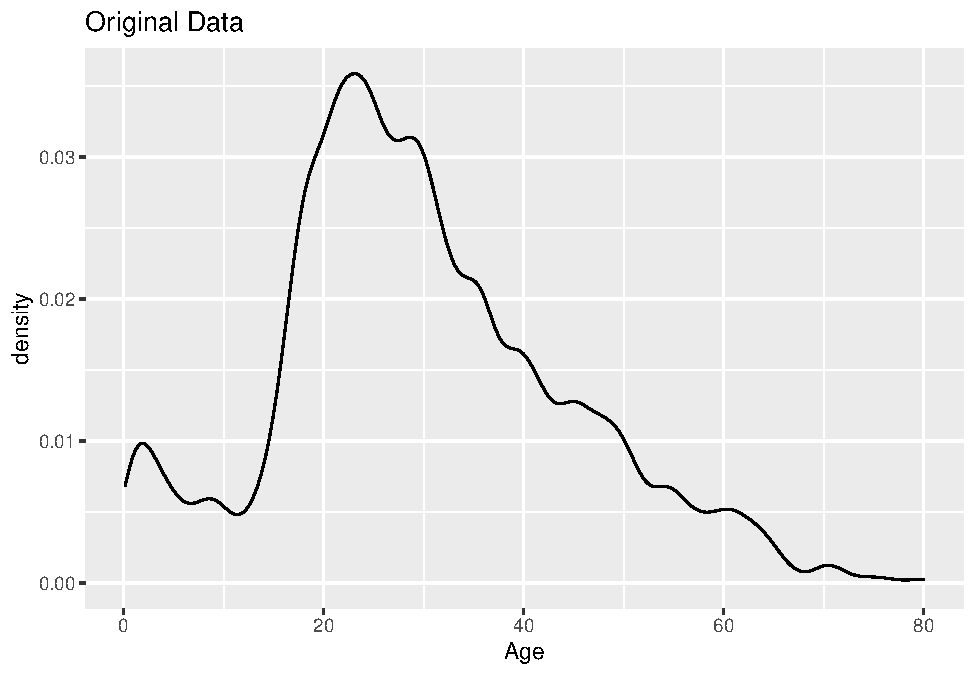
\includegraphics{titanic-analysis_files/figure-latex/pplot-1.pdf}
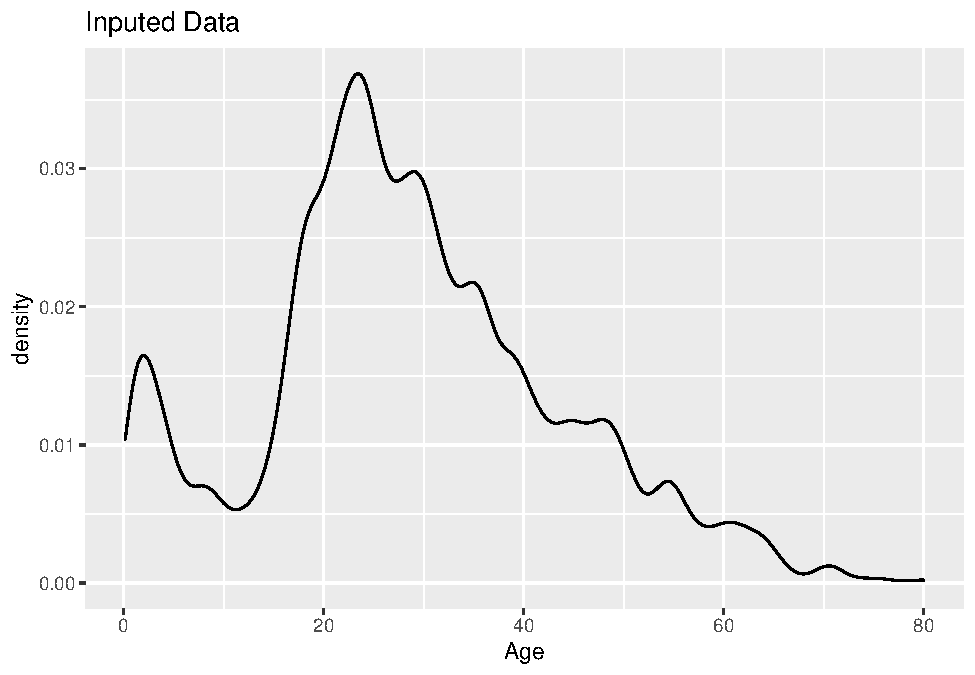
\includegraphics{titanic-analysis_files/figure-latex/pplot-2.pdf}

Observem que els dos gràfics són raonablement semblants, per tant
procedim a reemplaçar les dades dels valors inputats als originals.

\begin{Shaded}
\begin{Highlighting}[]
\CommentTok{\# Insertem a la columna \textquotesingle{}Age\textquotesingle{} del dataset original la nova columna calculada amb la lliberia \textquotesingle{}mice\textquotesingle{}}
\NormalTok{dataset}\SpecialCharTok{$}\NormalTok{Age }\OtherTok{\textless{}{-}}\NormalTok{ trained\_mouse}\SpecialCharTok{$}\NormalTok{Age}
\end{Highlighting}
\end{Shaded}

\hypertarget{ajust-de-la-variable-embarked.}{%
\subsubsection{Ajust de la variable
`Embarked'.}\label{ajust-de-la-variable-embarked.}}

Com hem vist anteriorment, hi ha dos valors de la variable
\textbf{Embarked} que falten. Per trobar el valor d'aquestes dues
observacions, procedim a verificar-ho amb l'ajuda dels valors de la
variable \textbf{Cabin}.

A partir de les dades, podem comprobar que totes les cabines que
comencen amb \textbf{B} es van embarcar des de les ciutats de
Southampton o Charbourg.

\begin{Shaded}
\begin{Highlighting}[]
\CommentTok{\# Mostrem els valors únics de la variable \textquotesingle{}Embark\textquotesingle{} quan el nom de la cabina comença per \textquotesingle{}B\textquotesingle{}}
\FunctionTok{unique}\NormalTok{(dataset[}\FunctionTok{grep}\NormalTok{(}\StringTok{"*\^{}B"}\NormalTok{, dataset}\SpecialCharTok{$}\NormalTok{Cabin),]}\SpecialCharTok{$}\NormalTok{Embarked)}
\end{Highlighting}
\end{Shaded}

\begin{verbatim}
## [1] C   S
## Levels:  C Q S
\end{verbatim}

A més a més, podem veure que els bitllets de viatge de tipus \textbf{B}
costen al voltant de 80 USD, que és molt similar a la tarifa mitja o
mitjana dels passatgers \textbf{S}.

\begin{Shaded}
\begin{Highlighting}[]
\CommentTok{\# Calcul de la mitja i la mitjana de les cabines que comencen per \textquotesingle{}B\textquotesingle{} (agrupat pels valors de la variable \textquotesingle{}Embark\textquotesingle{})}
\NormalTok{dataset[}\FunctionTok{grep}\NormalTok{(}\StringTok{"*\^{}B"}\NormalTok{, dataset}\SpecialCharTok{$}\NormalTok{Cabin),] }\SpecialCharTok{\%\textgreater{}\%} \FunctionTok{group\_by}\NormalTok{(Embarked) }\SpecialCharTok{\%\textgreater{}\%} \FunctionTok{summarize\_each}\NormalTok{(}\FunctionTok{funs}\NormalTok{(mean),Fare)}
\end{Highlighting}
\end{Shaded}

\begin{verbatim}
## # A tibble: 3 x 2
##   Embarked  Fare
##   <fct>    <dbl>
## 1 ""        80  
## 2 "C"      167. 
## 3 "S"       78.6
\end{verbatim}

\begin{Shaded}
\begin{Highlighting}[]
\NormalTok{dataset[}\FunctionTok{grep}\NormalTok{(}\StringTok{"*\^{}B"}\NormalTok{, dataset}\SpecialCharTok{$}\NormalTok{Cabin),] }\SpecialCharTok{\%\textgreater{}\%} \FunctionTok{group\_by}\NormalTok{(Embarked) }\SpecialCharTok{\%\textgreater{}\%} \FunctionTok{summarize\_each}\NormalTok{(}\FunctionTok{funs}\NormalTok{(median),Fare)}
\end{Highlighting}
\end{Shaded}

\begin{verbatim}
## # A tibble: 3 x 2
##   Embarked  Fare
##   <fct>    <dbl>
## 1 ""        80  
## 2 "C"       91.1
## 3 "S"       82.3
\end{verbatim}

Per tant, procedim a inputar els dos valors perduts de \textbf{Embarked}
com a tipus \textbf{S}.

\begin{Shaded}
\begin{Highlighting}[]
\CommentTok{\# Inputem el valor \textquotesingle{}S\textquotesingle{} en les dues observacions amb valors buits}
\NormalTok{dataset}\SpecialCharTok{$}\NormalTok{Embarked[}\FunctionTok{c}\NormalTok{(}\DecValTok{62}\NormalTok{, }\DecValTok{830}\NormalTok{)] }\OtherTok{\textless{}{-}} \StringTok{\textquotesingle{}S\textquotesingle{}}
\end{Highlighting}
\end{Shaded}

\hypertarget{ajust-de-la-variable-fare.}{%
\subsubsection{Ajust de la variable
`Fare'.}\label{ajust-de-la-variable-fare.}}

En aquest cas, com només es tracta d'un registre que no conté la dada,
el que farem serà introduïr la mitjana de la resta de valors d'aquesta
columna. Aquesta tècnica d'inputació de dades és molt freqüent quan la
quantitat de valors no informats és petita i quan l'atribut és del tipus
numèric.

Primer de tot, busquem on està localitzat el valor perdut de la variable
\textbf{Fare}.

\begin{Shaded}
\begin{Highlighting}[]
\CommentTok{\# Trobem quina és la posició de l\textquotesingle{}observació que conté el valor buit/NULL}
\FunctionTok{which}\NormalTok{(}\FunctionTok{is.na}\NormalTok{(dataset}\SpecialCharTok{$}\NormalTok{Fare))}
\end{Highlighting}
\end{Shaded}

\begin{verbatim}
## [1] 1044
\end{verbatim}

A continuació, trobem la mitjana del total dels tiquets excloent el
valor perdut.

\begin{Shaded}
\begin{Highlighting}[]
\CommentTok{\# Calculem la mitjana dels valors de la columna \textquotesingle{}Fare\textquotesingle{} eliminant el registre amb valor buit}
\NormalTok{mean\_fare }\OtherTok{\textless{}{-}} \FunctionTok{mean}\NormalTok{(dataset}\SpecialCharTok{$}\NormalTok{Fare, }\AttributeTok{na.rm =} \ConstantTok{TRUE}\NormalTok{)}
\end{Highlighting}
\end{Shaded}

Per últim, inputem el el valor obtingut al valor perdut de la columna
\textbf{Fare}.

\begin{Shaded}
\begin{Highlighting}[]
\CommentTok{\# Definim el valor de l\textquotesingle{}observació número \textquotesingle{}1044\textquotesingle{} amb el valor de la mitjana abans calculat}
\NormalTok{dataset}\SpecialCharTok{$}\NormalTok{Fare[}\FunctionTok{c}\NormalTok{(}\DecValTok{1044}\NormalTok{)] }\OtherTok{\textless{}{-}}\NormalTok{ mean\_fare}
\end{Highlighting}
\end{Shaded}

\hypertarget{comprovaciuxf3-de-valors-buits.}{%
\subsubsection{Comprovació de valors
buits.}\label{comprovaciuxf3-de-valors-buits.}}

Com podem observar en el càlcul que computarem a continuació, la
quantitat de valors no informats després del tractament és de zero
observacions.

\begin{Shaded}
\begin{Highlighting}[]
\CommentTok{\# Mostrem el número de registres buits per cada columna }
\FunctionTok{apply}\NormalTok{(dataset}\SpecialCharTok{==}\StringTok{""}\NormalTok{,}\DecValTok{2}\NormalTok{, sum)}
\end{Highlighting}
\end{Shaded}

\begin{verbatim}
## PassengerId    Survived      Pclass        Name         Sex         Age 
##           0           0           0           0           0           0 
##       SibSp       Parch      Ticket        Fare       Cabin    Embarked 
##           0           0           0           0        1014           0 
##    row_type 
##           0
\end{verbatim}

\begin{Shaded}
\begin{Highlighting}[]
\FunctionTok{apply}\NormalTok{(}\FunctionTok{is.na}\NormalTok{(dataset),}\DecValTok{2}\NormalTok{, sum)}
\end{Highlighting}
\end{Shaded}

\begin{verbatim}
## PassengerId    Survived      Pclass        Name         Sex         Age 
##           0           0           0           0           0           0 
##       SibSp       Parch      Ticket        Fare       Cabin    Embarked 
##           0           0           0           0           0           0 
##    row_type 
##           0
\end{verbatim}

\hypertarget{valors-extrems-outliers.}{%
\subsection{Valors extrems (outliers).}\label{valors-extrems-outliers.}}

L'estudi de valors extrem el farem només en les variables del tipus
quantitatiu. Això és així ja que, per les variables del tipus
qualitatiu, és molt difícil saber que vol dir que un valor esta fora del
que es considera `normal' (o similar a la resta).

\hypertarget{identificaciuxf3-de-les-columnes-amb-valors-extrems}{%
\subsubsection{Identificació de les columnes amb valors
extrems}\label{identificaciuxf3-de-les-columnes-amb-valors-extrems}}

A continuació, passem a mostrar una sèrie de gràfiques i taules
d'estadístiques que ens ajudaran a identificar aquells atributs amb
valors extrems.

\begin{Shaded}
\begin{Highlighting}[]
\CommentTok{\# Mostrem l\textquotesingle{}histograma i un resum de la variable \textquotesingle{}Survived\textquotesingle{}}
\FunctionTok{hist}\NormalTok{(dataset}\SpecialCharTok{$}\NormalTok{Survived, }\AttributeTok{col =} \StringTok{"blue"}\NormalTok{)}
\end{Highlighting}
\end{Shaded}

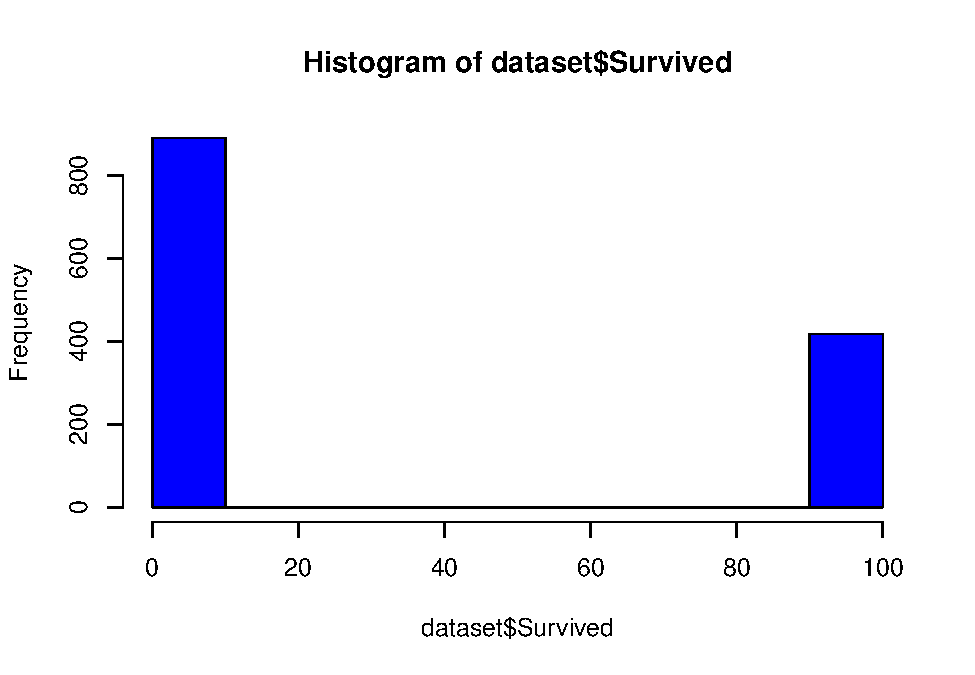
\includegraphics{titanic-analysis_files/figure-latex/unnamed-chunk-14-1.pdf}

\begin{Shaded}
\begin{Highlighting}[]
\FunctionTok{summary}\NormalTok{(dataset}\SpecialCharTok{$}\NormalTok{Survived)}
\end{Highlighting}
\end{Shaded}

\begin{verbatim}
##    Min. 1st Qu.  Median    Mean 3rd Qu.    Max. 
##    0.00    0.00    1.00   31.87   99.00   99.00
\end{verbatim}

\begin{Shaded}
\begin{Highlighting}[]
\FunctionTok{table}\NormalTok{(dataset}\SpecialCharTok{$}\NormalTok{Survived)}
\end{Highlighting}
\end{Shaded}

\begin{verbatim}
## 
##   0   1  99 
## 549 342 418
\end{verbatim}

\begin{Shaded}
\begin{Highlighting}[]
\CommentTok{\# Mostrem l\textquotesingle{}histograma i un resum de la variable \textquotesingle{}Survived\textquotesingle{}}
\FunctionTok{hist}\NormalTok{(dataset}\SpecialCharTok{$}\NormalTok{Pclass, }\AttributeTok{col =} \StringTok{"blue"}\NormalTok{)}
\end{Highlighting}
\end{Shaded}

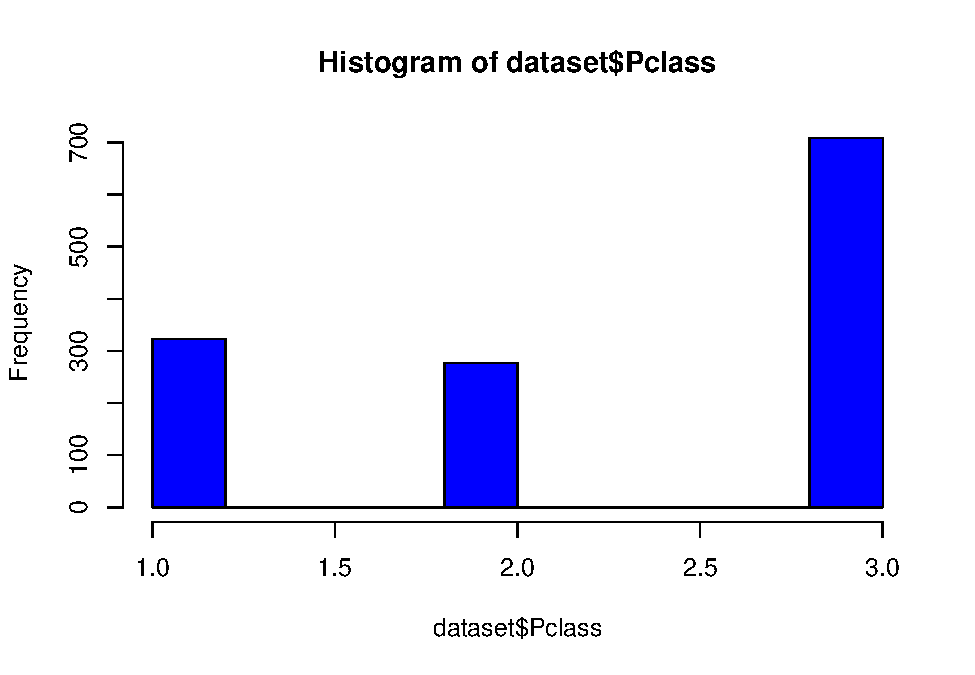
\includegraphics{titanic-analysis_files/figure-latex/unnamed-chunk-14-2.pdf}

\begin{Shaded}
\begin{Highlighting}[]
\FunctionTok{summary}\NormalTok{(dataset}\SpecialCharTok{$}\NormalTok{Pclass)}
\end{Highlighting}
\end{Shaded}

\begin{verbatim}
##    Min. 1st Qu.  Median    Mean 3rd Qu.    Max. 
##   1.000   2.000   3.000   2.295   3.000   3.000
\end{verbatim}

\begin{Shaded}
\begin{Highlighting}[]
\FunctionTok{table}\NormalTok{(dataset}\SpecialCharTok{$}\NormalTok{Pclass)}
\end{Highlighting}
\end{Shaded}

\begin{verbatim}
## 
##   1   2   3 
## 323 277 709
\end{verbatim}

\begin{Shaded}
\begin{Highlighting}[]
\CommentTok{\# Mostrem l\textquotesingle{}histograma i un resum de la variable \textquotesingle{}Age\textquotesingle{}}
\FunctionTok{hist}\NormalTok{(dataset}\SpecialCharTok{$}\NormalTok{Age, }\AttributeTok{col =} \StringTok{"blue"}\NormalTok{)}
\end{Highlighting}
\end{Shaded}

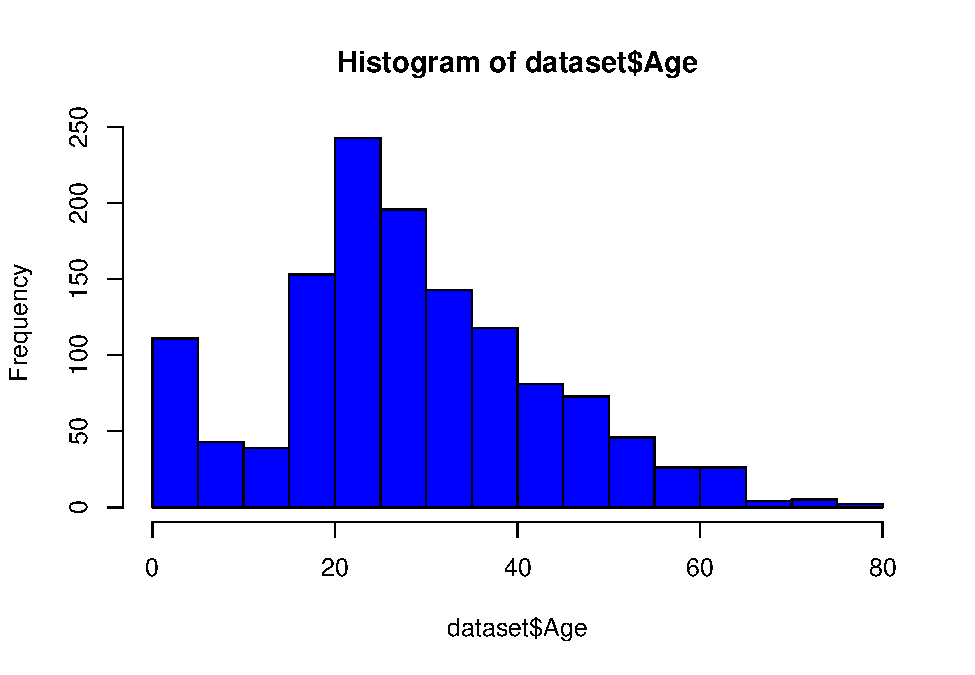
\includegraphics{titanic-analysis_files/figure-latex/unnamed-chunk-14-3.pdf}

\begin{Shaded}
\begin{Highlighting}[]
\FunctionTok{summary}\NormalTok{(dataset}\SpecialCharTok{$}\NormalTok{Age)}
\end{Highlighting}
\end{Shaded}

\begin{verbatim}
##    Min. 1st Qu.  Median    Mean 3rd Qu.    Max. 
##    0.17   20.00   27.00   28.70   38.00   80.00
\end{verbatim}

\begin{Shaded}
\begin{Highlighting}[]
\CommentTok{\# Mostrem l\textquotesingle{}histograma i un resum de la variable \textquotesingle{}SibSp\textquotesingle{}}
\FunctionTok{hist}\NormalTok{(dataset}\SpecialCharTok{$}\NormalTok{SibSp, }\AttributeTok{col =} \StringTok{"blue"}\NormalTok{)}
\end{Highlighting}
\end{Shaded}

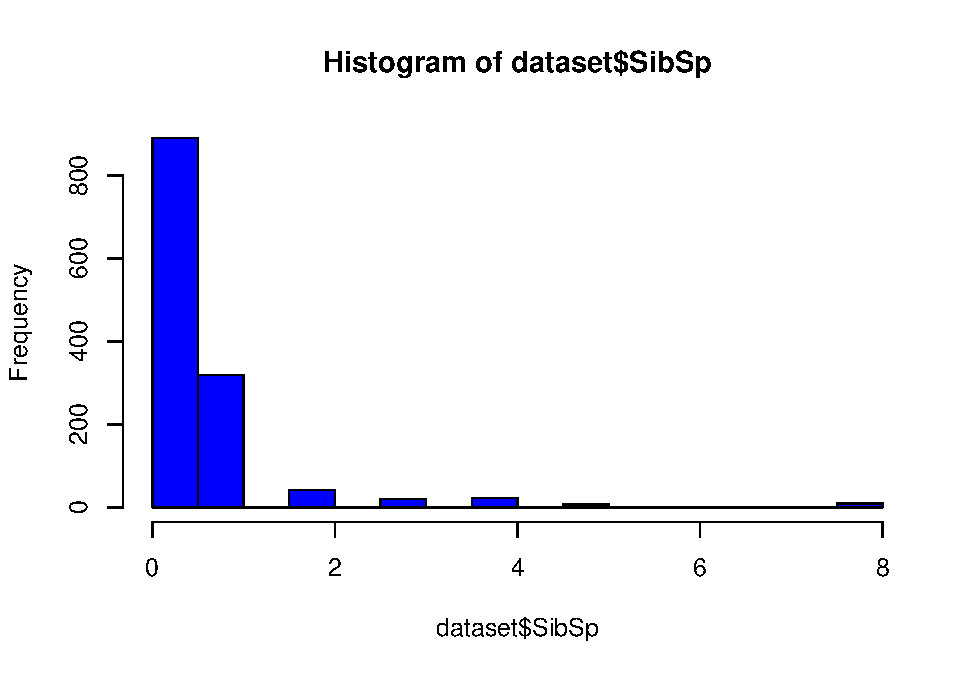
\includegraphics{titanic-analysis_files/figure-latex/unnamed-chunk-14-4.pdf}

\begin{Shaded}
\begin{Highlighting}[]
\FunctionTok{summary}\NormalTok{(dataset}\SpecialCharTok{$}\NormalTok{SibSp)}
\end{Highlighting}
\end{Shaded}

\begin{verbatim}
##    Min. 1st Qu.  Median    Mean 3rd Qu.    Max. 
##  0.0000  0.0000  0.0000  0.4989  1.0000  8.0000
\end{verbatim}

\begin{Shaded}
\begin{Highlighting}[]
\FunctionTok{table}\NormalTok{(dataset}\SpecialCharTok{$}\NormalTok{SibSp)}
\end{Highlighting}
\end{Shaded}

\begin{verbatim}
## 
##   0   1   2   3   4   5   8 
## 891 319  42  20  22   6   9
\end{verbatim}

\begin{Shaded}
\begin{Highlighting}[]
\CommentTok{\# Mostrem l\textquotesingle{}histograma i un resum de la variable \textquotesingle{}Parch\textquotesingle{}}
\FunctionTok{hist}\NormalTok{(dataset}\SpecialCharTok{$}\NormalTok{Parch, }\AttributeTok{col =} \StringTok{"blue"}\NormalTok{)}
\end{Highlighting}
\end{Shaded}

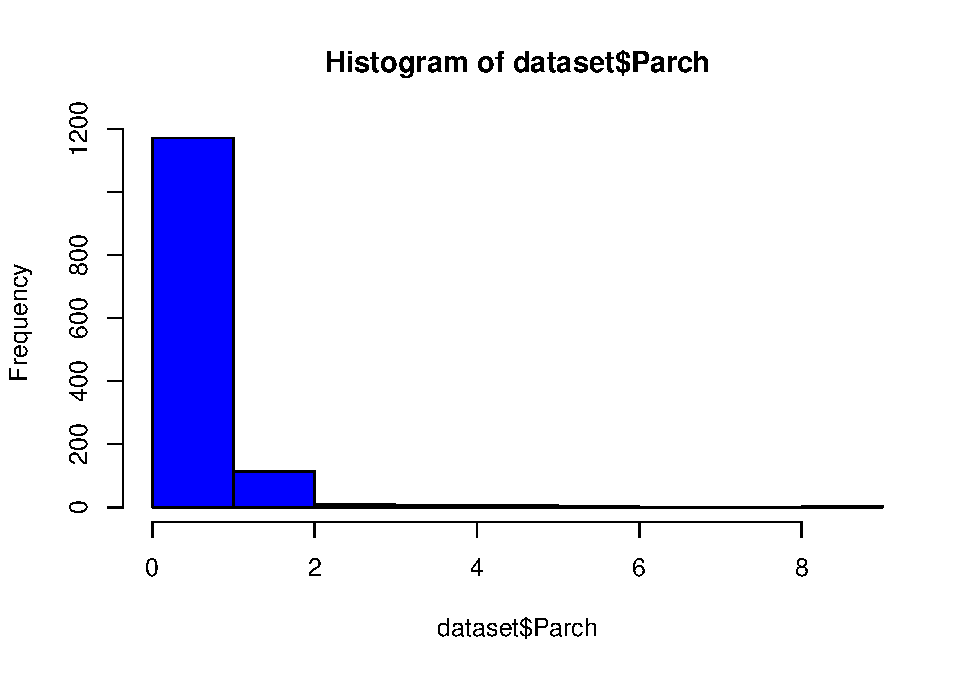
\includegraphics{titanic-analysis_files/figure-latex/unnamed-chunk-14-5.pdf}

\begin{Shaded}
\begin{Highlighting}[]
\FunctionTok{summary}\NormalTok{(dataset}\SpecialCharTok{$}\NormalTok{Parch)}
\end{Highlighting}
\end{Shaded}

\begin{verbatim}
##    Min. 1st Qu.  Median    Mean 3rd Qu.    Max. 
##   0.000   0.000   0.000   0.385   0.000   9.000
\end{verbatim}

\begin{Shaded}
\begin{Highlighting}[]
\FunctionTok{table}\NormalTok{(dataset}\SpecialCharTok{$}\NormalTok{Parch)}
\end{Highlighting}
\end{Shaded}

\begin{verbatim}
## 
##    0    1    2    3    4    5    6    9 
## 1002  170  113    8    6    6    2    2
\end{verbatim}

\begin{Shaded}
\begin{Highlighting}[]
\CommentTok{\# Mostrem l\textquotesingle{}histograma i un resum de la variable \textquotesingle{}Fare\textquotesingle{}}
\FunctionTok{hist}\NormalTok{(dataset}\SpecialCharTok{$}\NormalTok{Fare, }\AttributeTok{col =} \StringTok{"blue"}\NormalTok{)}
\end{Highlighting}
\end{Shaded}

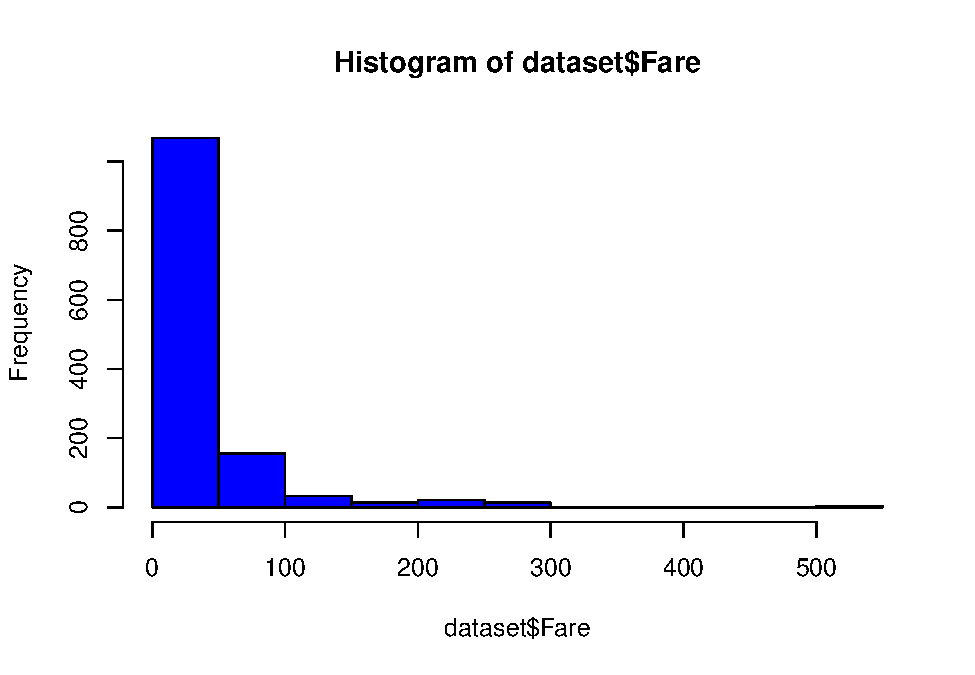
\includegraphics{titanic-analysis_files/figure-latex/unnamed-chunk-14-6.pdf}

\begin{Shaded}
\begin{Highlighting}[]
\FunctionTok{summary}\NormalTok{(dataset}\SpecialCharTok{$}\NormalTok{Fare)}
\end{Highlighting}
\end{Shaded}

\begin{verbatim}
##    Min. 1st Qu.  Median    Mean 3rd Qu.    Max. 
##   0.000   7.896  14.454  33.295  31.275 512.329
\end{verbatim}

D'aquesta informació, observem el següent:

\begin{itemize}
\item
  \textbf{Survived}: Tots els valors són o bé 0 o bé 1. Els valors 99
  són els que hem inputat nosaltres quan hem fet el \emph{merge} del joc
  de dades de `test' amb el de `train'. No hi ha cap fora dels valors
  esperats i, per tant, no eliminarem cap registre en base a aquest
  atribut.
\item
  \textbf{Pclass}: Tots els valors són o bé 1 o bé 2 o bé 3. Les
  diferents classes de tiquet. No hi ha cap fora dels valors esperats i,
  per tant, no eliminarem cap registre en base a aquest atribut.
\item
  \textbf{Age}: El mínim és 0.17 i el màxim és 80. No hi ha cap edat que
  cridi l'atenció com per considerar-la fora de l'esperat i eliminar-la
  del joc de dades.
\item
  \textbf{SibSp}: Gran part dels valors són enters entre 0 i 1. Hi ha un
  9 observacions amb un valor allunyat de la resta com és el valor 8.
  Tot i això, és un valor que seria possible ja que existeixen families
  numerosas amb aquesta quantitat de fills. En el nostre cas, no
  eliminarem aquestes observacions ja que no les considerem extremes
  (tot i que sí poc probables).
\item
  \textbf{Parch}: Gran part dels valors són enters entre 0 i 1. Hi ha 2
  observacions amb un valor allunyat de la resta com és el valor 9. Tot
  i això, és un valor que seria possible ja que existeixen families
  numerosas amb aquesta quantitat de fills. En el nostre cas, no
  eliminarem aquestes observacions ja que no les considerem extremes
  (tot i que sí poc probables).
\item
  \textbf{Fare}: Existeixen 4 observacions amb un valor extremadament
  allunyat de la resta. Aquest valor és el valor 512.329 que és el màxim
  de la variable. Com hem pogut observar al resum d'estadístiques, la
  mitjana dels valors d'aquesta columna és 33.295, és a dir, es troba
  molt lluny de la tendència de valors (també de la mediana i dels
  quartils). És per aquest motiu que eliminarem aquesta observació i
  recalcularem la mitjana per introduïrla en els valors que originalment
  eren buits (ja que abans ho haviem fet amb una mitjana esbiaixada).
\end{itemize}

Cal apuntar que tot i que hi hagi d'altres valors de la variable
\textbf{Fare} que semblin extrems, creiem que es poden arribar a donar i
és per aquest motiu que els mantindrem.

\hypertarget{ajust-de-la-variable-fare}{%
\subsubsection{Ajust de la variable
`Fare'}\label{ajust-de-la-variable-fare}}

A continuació eliminarem el registre que conté el valor extrem en la
variable \textbf{Fare} i recalcularem la mitjana per introduïrla en els
valors que originalment eren buits (ja que abans ho haviem fet amb una
mitjana esbiaixada).

\begin{Shaded}
\begin{Highlighting}[]
\CommentTok{\# Calculem el màxim de la variable \textquotesingle{}Fare\textquotesingle{}}
\NormalTok{max\_fare }\OtherTok{\textless{}{-}} \FunctionTok{max}\NormalTok{(dataset}\SpecialCharTok{$}\NormalTok{Fare)}

\CommentTok{\# Mostrem les dimensions del \textquotesingle{}dataset\textquotesingle{} abans d\textquotesingle{}eliminar les observacions}
\FunctionTok{dim}\NormalTok{(dataset)}
\end{Highlighting}
\end{Shaded}

\begin{verbatim}
## [1] 1309   13
\end{verbatim}

\begin{Shaded}
\begin{Highlighting}[]
\CommentTok{\# Eliminem els registres on el valor és igual al màxim }
\NormalTok{dataset }\OtherTok{\textless{}{-}}\NormalTok{ dataset[dataset}\SpecialCharTok{$}\NormalTok{Fare }\SpecialCharTok{!=}\NormalTok{ max\_fare,]}

\CommentTok{\# Mostrem les dimensions del \textquotesingle{}dataset\textquotesingle{} després d\textquotesingle{}eliminar les observacions}
\FunctionTok{dim}\NormalTok{(dataset)}
\end{Highlighting}
\end{Shaded}

\begin{verbatim}
## [1] 1305   13
\end{verbatim}

\begin{Shaded}
\begin{Highlighting}[]
\CommentTok{\# Calculem el màxim de la variable \textquotesingle{}Fare\textquotesingle{}}
\FunctionTok{max}\NormalTok{(dataset}\SpecialCharTok{$}\NormalTok{Fare)}
\end{Highlighting}
\end{Shaded}

\begin{verbatim}
## [1] 263
\end{verbatim}

\begin{Shaded}
\begin{Highlighting}[]
\CommentTok{\# Calculem la mitjana de la variable \textquotesingle{}Fare\textquotesingle{}}
\NormalTok{mean\_fare }\OtherTok{\textless{}{-}} \FunctionTok{mean}\NormalTok{(dataset}\SpecialCharTok{$}\NormalTok{Fare)}

\CommentTok{\# Introduïm el nou valor en l\textquotesingle{}observació que originalment era buida (l\textquotesingle{}observació 1044)}
\NormalTok{dataset}\SpecialCharTok{$}\NormalTok{Fare[}\FunctionTok{c}\NormalTok{(}\DecValTok{1044}\NormalTok{)] }\OtherTok{\textless{}{-}}\NormalTok{ mean\_fare}
\end{Highlighting}
\end{Shaded}

\hypertarget{altres-accions-per-a-la-neteja-del-joc-de-dades.}{%
\subsection{Altres accions per a la neteja del joc de
dades.}\label{altres-accions-per-a-la-neteja-del-joc-de-dades.}}

Primerament, observem que la primera variable ``PassengerId'' no és res
més que un identificador, per tant procedim a eliminar-la del conjunt de
dades ja que no ens interessa per l'estudi.

\begin{Shaded}
\begin{Highlighting}[]
\CommentTok{\# eliminació de la primera columna PassengerId}
\FunctionTok{dim}\NormalTok{(}\FunctionTok{unique}\NormalTok{(dataset}\SpecialCharTok{$}\NormalTok{PassengerId))}
\end{Highlighting}
\end{Shaded}

\begin{verbatim}
## NULL
\end{verbatim}

\begin{Shaded}
\begin{Highlighting}[]
\NormalTok{dataset }\OtherTok{\textless{}{-}}\NormalTok{ dataset[,}\SpecialCharTok{{-}}\DecValTok{1}\NormalTok{]}
\end{Highlighting}
\end{Shaded}

Observem que les variables `Survived' i `Pclass' són de tipus enter,
però la seva funció es indicar una categoria. Per tant, procedim a
convertir-les en tipu factor.

\begin{Shaded}
\begin{Highlighting}[]
\CommentTok{\# transformació de les variables }

\NormalTok{dataset}\SpecialCharTok{$}\NormalTok{Survived }\OtherTok{\textless{}{-}} \FunctionTok{as.factor}\NormalTok{(dataset}\SpecialCharTok{$}\NormalTok{Survived)}
\FunctionTok{class}\NormalTok{(dataset}\SpecialCharTok{$}\NormalTok{Survived)}
\end{Highlighting}
\end{Shaded}

\begin{verbatim}
## [1] "factor"
\end{verbatim}

\begin{Shaded}
\begin{Highlighting}[]
\NormalTok{dataset}\SpecialCharTok{$}\NormalTok{Pclass }\OtherTok{\textless{}{-}} \FunctionTok{as.factor}\NormalTok{(dataset}\SpecialCharTok{$}\NormalTok{Pclass)}
\FunctionTok{class}\NormalTok{(dataset}\SpecialCharTok{$}\NormalTok{Pclass)}
\end{Highlighting}
\end{Shaded}

\begin{verbatim}
## [1] "factor"
\end{verbatim}

\hypertarget{anuxe0lisi-de-les-dades.}{%
\section{Anàlisi de les dades.}\label{anuxe0lisi-de-les-dades.}}

\hypertarget{selecciuxf3-de-grups-a-analitzarcomparar.}{%
\subsection{Selecció de grups a
analitzar/comparar.}\label{selecciuxf3-de-grups-a-analitzarcomparar.}}

\begin{Shaded}
\begin{Highlighting}[]
\CommentTok{\# Placeholder}
\end{Highlighting}
\end{Shaded}

\hypertarget{normalitat-i-homogeneuxeftat-de-la-variuxe0ncia.}{%
\subsection{Normalitat i homogeneïtat de la
variància.}\label{normalitat-i-homogeneuxeftat-de-la-variuxe0ncia.}}

\begin{Shaded}
\begin{Highlighting}[]
\CommentTok{\# Placeholder}
\end{Highlighting}
\end{Shaded}

\hypertarget{aplicaciuxf3-de-proves-estaduxedstiques-per-a-la-comparaciuxf3-de-grups.}{%
\subsection{Aplicació de proves estadístiques per a la comparació de
grups.}\label{aplicaciuxf3-de-proves-estaduxedstiques-per-a-la-comparaciuxf3-de-grups.}}

\begin{Shaded}
\begin{Highlighting}[]
\CommentTok{\# Placeholder}
\end{Highlighting}
\end{Shaded}

\hypertarget{representaciuxf3-de-resultats-taules-i-gruxe0fiques.}{%
\section{Representació de resultats (taules i
gràfiques).}\label{representaciuxf3-de-resultats-taules-i-gruxe0fiques.}}

\begin{Shaded}
\begin{Highlighting}[]
\CommentTok{\# Placeholder}
\end{Highlighting}
\end{Shaded}

\hypertarget{conclusions.}{%
\section{Conclusions.}\label{conclusions.}}

\end{document}
